% !TeX spellcheck = en_US
\documentclass[conference]{IEEEtran}
\usepackage[utf8]{inputenc}
\usepackage[english]{babel}
\usepackage{amsfonts}
\usepackage{amsmath}
\usepackage{breqn}
\usepackage{cite}
\usepackage{graphicx}


%s\usepackage{draftwatermark}
\IEEEoverridecommandlockouts	
\begin{document}
	
%\title{Improving Uplink Capacity in IEEE 802.11ax Networks}
\title{Proportional Fair Uplink Scheduler for IEEE~802.11ax: a Classic Problem with New Constraints  \thanks{The research was supported by the Russian Science Foundation (agreement No 16-19-10687).}}

%Анализ эффективности механизма доступа к среде при использовании триггер-кадров в сетях Wi-Fi нового поколения.


\author{\IEEEauthorblockN{ Evgeny Khorov \IEEEauthorrefmark{2}\IEEEauthorrefmark{1}, Vyacheslav Loginov \IEEEauthorrefmark{1} and Andrey Lyakhov \IEEEauthorrefmark{1}}
	\IEEEauthorblockN{\IEEEauthorrefmark{1} Institute for Information Transmission Problems, Russian Academy of Sciences, Moscow, Russia\\Email: loginov@iitp.ru}
	\IEEEauthorblockN{\IEEEauthorrefmark{2} Skolkovo Institute of Science and Technology, Moscow, Russia\\Email: e@khorov.ru}
}
%\author{ Evgeny Khorov\IEEEauthorrefmark{1}, Vyacheslav Loginov\IEEEauthorrefmark{1}, Andrey Lyakhov\IEEEauthorrefmark{1}, \\\IEEEauthorrefmark{1}Institute for Information Transmission Problems, Russian Academy of Sciences, Moscow, Russia\\\IEEEauthorrefmark{2}Quantenna Communications, US\\Email: \{ khorov, loginov, lyakhov\}@iitp.ru, sschelstraete@quantenna.com 
%}

\maketitle

\begin{abstract}
	To improve efficiency of spectrum usage in different scenarios, Wi-Fi community is currently developing a new standard, namely IEEE 802.11ax. 
	Its main feature is OFDMA. Apart from obvious advantages, such as decreasing overhead for short packet transmission at high rates and improving robustness to fading and interference, being used for uplink transmission, OFDMA can increase power spectral density and thus increase user data rates. The gain of OFDMA is mainly depends on how the resources are scheduled between users. In the paper, we study the scheduling problem in 11ax, paying much attention to those peculiarities which make 11ax OFDMA differ from that of LTE. Then we adapt well-known proportional fair scheduler to 802.11ax and evaluate how much it improves throughout for uplink transmission.
	
%	The latter results in higher throughput.   
%	
%	To cope with raising number of Wi-Fi devices, the new amendment IEEE 802.11ax for the Wi-Fi standard is being developed. One of the major improvements, which 802.11ax brings to Wi-Fi, is  OFDMA in addition to the legacy OFDM. Being designed for dense networks, 802.11ax provides flexible framework for resource allocation with OFDMA allowing to serve multiple users simultaneously. However, the new amendment does not provide any scheduling algorithm needed for OFDMA operation. In this paper, we compare OFDMA schemes used in Wi-Fi and LTE, and estimate the performance of 802.11ax uplink OFDMA with different scheduling algorithms.
	
\end{abstract}
\begin{IEEEkeywords}
	High Efficiency WLANs, IEEE 802.11ax, OFDMA, performance evaluation, scheduling algorithm.
\end{IEEEkeywords}

%\IEEEpeerreviewmaketitle
\section{Introduction}
\label{intro}
%- IEEE 802.11ax introduces OFDMA to Wi-Fi

%In contrast to 11ac which 10 times increased the maximal data rates 


%Allows simultaneous low-data-rate transmission from several users.
%Pulsed carrier can be avoided.
%Lower maximum transmission power for low data rate users.
%Shorter delay, and constant delay.
%Contention-based multiple access (collision avoidance) is simplified.
%Further improves OFDM robustness to fading and interference.
%Combat narrow-band interference.
%Claimed OFDMA Advantages[edit]
%Flexibility of deployment across various frequency bands with little needed modification to the air interface.[1]
%Averaging interferences from neighboring cells, by using different basic carrier permutations between users in different cells.
%Interferences within the cell are averaged by using allocation with cyclic permutations.
%Enables Single Frequency Network coverage, where coverage problem exists and gives excellent coverage.
%Offers Frequency diversity by spreading the carriers all over the used spectrum.
%Allows per channel or per subchannel power
%Recognised disadvantages of OFDMA[edit]
%Higher sensitivity to frequency offsets and phase noise.[1]
%Asynchronous data communication services such as web access are characterised by short communication bursts at high data rate. Few users in a base station cell are transferring data simultaneously at low constant data rate.
%The complex OFDM electronics, including the FFT algorithm and forward error correction, are constantly active independent of the data rate, which is inefficient from power consumption point of view, while OFDM combined with data packet scheduling may allow FFT algorithm to hibernate during certain time intervals.
%The OFDM diversity gain, and resistance to frequency-selective fading, may partly be lost if very few sub-carriers are assigned to each user, and if the same carrier is used in every OFDM symbol. Adaptive sub-carrier assignment based on fast feedback information about the channel, or sub-carrier frequency hopping, is therefore desirable.
%Dealing with co-channel interference from nearby cells is more complex in OFDM than in CDMA. It would require dynamic channel allocation with advanced coordination among adjacent base stations.
%The fast channel feedback information and adaptive sub-carrier assignment is more complex than CDMA fast power control.


Nowadays, Wi-Fi has become the main technology for wireless local area networks. High number of Wi-Fi devices itself, and the number of deployed networks lead to huge interference. To improve efficiency of Wi-Fi networks in existing and emerging indoor and outdoor scenarios, Wi-Fi community is currently developing a new standard, namely IEEE 802.11ax. 

In contrast to 11ac, which 10 times increases the maximal data rates at the PHY layer, the gain of 11ax at the PHY layer is just 37\% (TODO check with Anton's paper), while for users the developers expect 4X gain thanks to new PHY and MAC techniques.     
%i access points (APs) and stations (STAs) is continuously increasing, so Wi-Fi networks become very dense. Due to the fact that Wi-Fi channel access is decentralized and contention-based, Wi-Fi performance in dense deployment scenarios may significantly degrade.

%To improve Wi-Fi efficacy in dense deployment scenarios, IEEE 802.11 working group, which standardize Wi-Fi, is preparing the new amendment called 802.11ax. 

The main feature of 11ax is the usage of  Orthogonal Frequency Division Multiple Access (OFDMA).  while legacy Wi-Fi uses CSMA/CA (CSMA/CA) and Orthogonal Frequency Division Multiplexing (OFDM). OFDMA is the multiuser version of OFDM which allows assigning non-overlapping sets of subcarriers to different users. As a result, devices can transmit data simultaneously without collisions.



%802.11ax introduces Orthogonal Frequency Division Multiple Access (OFDMA) to Wi-Fi in addition to legacy single-user Orthogonal Frequency Division Multiplexing (OFDM) modulation scheme. OFDMA is a promising technology being used in many other wireless networks, e.g. LTE and WiMax. With OFDMA, the AP can assign non overlapping sets of a subcarriers to different users and allow simultaneous transmission. 

One of the most important parts of OFDMA implementation which significantly affects network performance is the scheduling algorithm performing subcarrier assignment. As usual, 802.11ax provides flexible framework for OFDMA resource allocation, but it does not provide any scheduling algorithm for efficient usage of OFDMA.

In this paper, we compare OFDMA schemes in IEEE 802.11ax and LTE, and analyze problems which have to solve 802.11ax scheduling algorithm.

The rest of the paper is organized as follows.  Section~\ref{sec:ofdma} briefly describes the main features of OFDMA in 802.11ax. Section~\ref{sec:conclusion} concludes the paper. 

\section{OFDMA in Modern Network Technologies}
\label{sec:ofdma}

OFDMA  is based on single user OFDM modulation scheme. With an OFDM, the whole available channel bandwidth is divided into closely spaced non-overlapping orthogonal subcarriers. On each subcarrier, the data is transmitted using conventional modulation scheme, e.g. QPSK or QAM-16. One of the main important features of OFDM is the it has  high level of resistance to the frequency selective fading due to multipath without use of complicated equalization filters. 

OFDMA is the multiuser version of OFDM which allows assigning non-overlapping sets of subcarriers to different users. As a result, users can transmit data simultaneously without collisions.

Implementation of the OFDMA must take into account peculiarities of the network. In the following sections, we briefly describe differences in OFDMA implementations used in LTE, which is the most widespread 4G cellular network technology, and in upcoming 802.11ax networks. %Also, we highlight why already developed algorithm for LTE scheduling can not be directly used in 802.11ax.

\subsection{OFDMA in LTE}

Channel access in LTE is centralized and fully controlled by the LTE base station (eNB). In LTE, available channel resources are divided into transmission time intervals (TTI) of 1ms duration in time and into sets containing 12 neighbor subcarriers in frequency. The minimal amount of channel resources which can be allocated by the scheduling algorithm consists of 12 subcarriers with duration of 1 TTI and is called resource block (RB). 

In LTE, different versions of OFDMA are used in uplink and downlink. In the downlink ``pure'' OFDMA is used, which does not have any constraints on RB allocation, the eNB can allocate any subset of RB to any UE. As a result, scheduling algorithms usually allocate RBs independently in each TTI accordingly to the considered utility function.

TODO add inforamtion about frequency selective interference/fading, wide-band CQIs, sub-band CQIs

TODO Allocated resource blocks form a transport block, i.e. a block of data which is transmitted with the same MCS. 

TODO Sometimes it is worth to exclude several bad resource blocks from the transport block if they significantly reduce MCS.

In contrast to downlink tranmissions, uplink  ones use Single Carrier FDMA (SC-FDMA). Due to space limitation, we can not describe SC-FDMA in much detail. In general, SC-FDMA allows to achieve lower peak-to-average power ratio (PAPR) comparing to the ``pure'' OFDMA, what improves user equipment (UE) power efficiency. However, SC-FDMA has one important limitation which significantly affects the scheduling algorithm: the eNB can allocate only contiguous set of RBs for a particular user. As a result, scheduling algorithms for LTE uplink have to allocate all RBs in one TTI jointly, which significantly increases the algorithm's complexity.

\subsection{Main Features of OFDMA in IEEE 802.11ax}

%main peculiarities of OFDMA in Wi-Fi

%How it differs from LTE ones

%Why it can be fruitful

%One of the most loved Wi-Fi features is backward compatibility. Several Wi-Fi generations have passed (IEEE 802.11a/b/g/n/ac), but still different generation Wi-Fi devices are capable to efficiently and fairly share common radio resources.

In contrast to the LTE, legacy Wi-Fi devices use decentralized CSMA/CA based channel access method called Enhanced Distributed Channel Access (EDCA) and OFDM modulation. 

To maintain backward compatibility between different generation Wi-Fi devices,  OFDMA in the 802.11ax operates on top of the EDCA and OFDM. In the downlink, the AP first transmits OFDM preamble which can be read by all Wi-Fi devices, and only after that OFDMA payload is transmitted. As a result, despite the fact that legacy STAs are not able to decode OFDMA payload, they would not interrupt the OFDMA transmission.

In the uplink, in order to solicit the OFDMA transmission, the AP transmits a special trigger frame containing information about resource allocation for different STAs. After reception of the trigger frame, STAs for whom the resources were allocated first transmit common OFDM preamble, and after that the data in the allocated subcarriers using the MCS indicated in the trigger frame. 

With the OFDMA introduced in 802.11ax, AP can split the whole bandwidth into sets of OFDM subcarriers (or tones) called resource units (RUs). Each RU consists of 26, 52, 106, 242, 484, or 996 OFDM-tones. The whole 80MHz channel corresponds to 996-tone RU. Each wide RU can be split into two approximately twice-narrower RUs. In turn, each of them can be split again, separately from another one. The exceptions are 996-tone RU which can be split into 2 484-tone RUs and 1 26-tone RU, and 242-tone RU which can be split into 2 106-tone RU and 1 26-tone RU.

While in downlink OFDMA just allows AP to transmit data to multiple users simultaneously, OFDMA in the uplink provides more benefits. In particular, independently on the size of RU in which STA is transmitting, STA spends the same amount of power $P_0$. Because of that, with OFDMA the signal power density is increased, so MCS with higher data rate can be used for transmission in narrower RU. As a result, in contrast to LTE, in 802.11ax uplink transmission data rate in different RUs is non-additive, i.e. if a STA transmits in twice wider RU, it is not guaranteed that it achieves twice higher data rate. Moreover, in some cases the achieved data rate can be even smaller.

Due to the standard limitations, the AP can allocate not bigger than one RU for each station independently on the RU type.

%Data rates of MCSs used in the 802.11ax are indicated in Table~\ref{table:RUdatarate}.
%
%\begin{table}[t]
%	{\centering
%		\caption{\label{table:RUdatarate} Data rate of different RU types at each MCS in Mbps}
%		\begin{tabular}{|c|c|c|c|c|c|c|}
%			\hline
%			\textbf{MCS}	& 26-tone  & 52-tone  & 106-tone  & 242-tone  & 484-tone  & 996-tone  \\
%			\hline
%			0	&0.8	&1.7	&3.5	&8.1 & 16.3 &34		\\
%			1	&1.7	&3.3	&7.1	&16.3 & 32.5 &68.1		\\
%			2	&2.5	&5	&10.6	&24.4 & 48.8 &102.1		\\
%			3	&3.3	&6.7	&14.2	&32.5 & 65 &136.1		\\
%			4	&5	&10	&21.3	&48.8 & 97.5 &204.2		\\
%			5	&6.7	&13.3	&28.3	&65 & 130 &272.2		\\
%			6	&7.5	&15	&31.9	&73.1 & 146.3 &306.3		\\
%			7	&8.3	&16.7	&35.4	&81.3 & 162.5 &340.3		\\
%			8	&10	&20	&42.5	&97.5 & 195 &408.3		\\
%			9	&11.1	&22.2	&47.2	&108.3 & 216.7 &453.7		\\
%			10	& --	&--	&--	&121.9 & 243.8 &510.4		\\
%			11	& --	&--	&--	&135.4 & 270.8 &576.1		\\
%			\hline
%		\end{tabular}
%	}
%\end{table}

\subsection{Related works}

Despite the fact that 802.11ax amendment is expected to be finished by 2019, it has been already studied in the literature\cite{khorov2016joint, khorov2016several, karaca2016resource, ofdma-par1, ofdma-par2}.

In \cite{khorov2016several}, authors study the performance of the network consisting of the legacy and 802.11ax STAs. Authors propose an approach for optimal channel access parameter values selection, which guarantees fairness between legacy and 802.11ax and significantly increase the number of the OFDMA transmissions for 802.11ax STAs. However, model developed in \cite{khorov2016several} allows only estimate the number of the OFDMA transmissions in the network, but not the achievable data rate.

At the meetings of the 802.11ax task group (TGax), many studies on 802.11ax performance was presented, e.g. \cite{ofdma-par1, ofdma-par2}. However, despite many network topologies has been already studied, in all works presented in TGax only random scheduler with a static RU configuration is considered.

% \cite{karaca2016resource} -- minimum padding scheduler for 802.11ax

\subsection{Problem Statement}

Let us consider 802.11ax network consisting of 1 AP serving $N$ stations using OFDMA and operating in a channel with 80MHz bandwidth at 5GHz frequency. All the STAs are dropped uniformly within a circle with radius $R$, the AP is located in the center of the circle.

We consider uplink only full buffer traffic model. 

We assume that the AP have a perfect knowledge about channel condition for STAs. Using minimum input level sensitivity of the decoder provided in the standard and the received signal power, we assume that the STA is transmitting at the fastest MCS allowed by the received signal power.

To determine which MCS STA locating at the distance $d$ can use at each RU type, we use the 802.11ax pass loss model for the residential scenario~\cite{presentation_scenarios}.
%:
%\begin{align*}
%PL(d) &= 40.05 + 20 log_{10}(\frac{f_c}{2.4}) + 20 log_{10}(min(d, 5)) + \\
%&+ \mathbb{I}(d > 5) 35 log_{10}(\frac{d}{5}),
%\end{align*}
%where $PL$ is the signal loss expressed in dB, $d$ is the distance between devices in m,  $f_c$ is the central channel frequency in GHz.
%Finally, $\mathbb{I}(x)$ equals $1$ if $x$ is true and $0$, otherwise.
As a result, the received signal power $P(d)$ can be estimated as follows
\[P(d) = P_0 + 10 log_{10}(\frac{T}{996}) - PL(d),\]
where $P_0$ is the transmitting power, and $d$ is the distance between the STA and the AP, $T$ is a number of tones in RU, $PL$ is a pathloss at distance $d$.

In this paper, we investigate the 802.11ax network uplink performance with different OFDMA scheduling algorithms in terms of average data rate of OFDMA transmissions.




\section{Scheduling Approaches}

OFDMA scheduler in IEEE 802.11ax AP is responsible for solving two main problems. The first one is the selection of the appropriate RU configuration, i.e. how to split available subcarriers into RUs. 
%To determine particular RU configuration, we use the following notation: 
%\begin{equation}
%\vec V_i = [ n_{26}(i), n_{52}(i),n_{106}(i),n_{242}(i),n_{484}(i),n_{996}(i) ], \end{equation}
%where $V_i$ is the considered RU configuration, $n_x(i)$ is the number of $x$-tone RUs in RU configuration $\vec V_i$.
%All RU configurations must meet to the following constraints:
%
%\begin{enumerate}
%	\item $0\leq n_x(i) \leq n_x^{Max}$, where $n_x^{Max}$ is the maximum number of $x$-tone RUs in configuration (1 for 996-tone RU, 37 for 26-tone RU),
%	
%	\item Smaller size RU can be used only if the bigger size RU is split, so the following conditions must be met
%	
%	\begin{equation} n_{484} \leq 2- 2 \cdot n_{996}\end{equation}
%	
%	\begin{equation} n_{242} \leq 4 - 4\cdot n_{996} - 2 \cdot n_{484}\end{equation}
%	
%	\begin{equation} n_{106} \leq 8 - 8\cdot n_{996} - 4\cdot n_{484} - 2\cdot n_{242}\end{equation}
%	
%	\begin{equation} n_{52} \leq 16 - 16\cdot n_{996} - 8\cdot n_{484} - 4\cdot n_{242} - 2 \cdot n_{106}\end{equation}
%	
%	\begin{equation} n_{26} \leq 37 - 37\cdot n_{996} - 18\cdot n_{484} - 9\cdot n_{242} - 4\cdot n_{106} - 2 \cdot n_{52}\end{equation}
%	
%	\item  Total number of RUs in configuration should not exceed the number of stations $N$
%	
%	\[n_{26} + n_{52} + n_{106} + n_{242} + n_{484} + n_{996} \leq N\]
%	
%\end{enumerate}
%
%After that, we use filtering procedure and exclude out of the consideration configurations vector if we found another configuration vector, which will be definitely better in terms of performance than the first one. In particular, if for considered vector $V_i$ we found possible configuration $V_j$ which meet the following condition
%
%\[D= V_j-V_i\]
%
%\[D(k) \geq 0, \forall k \in [1,6]\]
%
%we exclude $V_i$ out of consideration.
RU configuration vectors are sorted as shown in Table~\ref{table:vectors}. 
%Configurations are sorted in ascending order using the following metric $$M(V_i) = \sum\limits_{k=1}^6 ( V_i(k)\cdot 10^{(2\cdot k)}).$$
\begin{table}[!tbp]
	\caption{\label{table:vectors} RU configuration vectors in lexical order}
	\centering
	\begin{tabular}{|l|l|l|l|l|l|l|}
		\hline
		\textbf{Configuration number}	& \textbf{$n_{996}$} & \textbf{$n_{484}$} & \textbf{$n_{242}$}  &  \textbf{$n_{106}$} & \textbf{$n_{52}$} & \textbf{$n_{26}$}  \\
		\hline
		1  & 0 & 0 & 0 &0 &0 &37\\
		2  & 0 & 0 & 0 &0 &1 &35\\
		3  & 0 & 0 & 0 &0 &2 &33\\
		..  & ..& .. & .. & .. & .. & ..\\
		16 & 0 & 0 & 0 &0 &15 &7\\
		17 & 0 & 0 & 0 &0 &16 &5\\
		18 & 0 & 0& 0 &1 &0 &33\\
		19 & 0&  0& 0& 1 &1 &31\\
    	20 & 0&  0& 0& 1 &2 &29\\
		..  & ..& .. & .. & .. & .. & ..\\
		200 & 0 & 1 & 1 & 2 &0 &2\\
		200 & 0 & 1 & 2 &0 &0 &1\\
		201 & 0& 2 & 0 &0 &0 &1\\
		202 & 1& 0 & 0 &0 &0 &0\\
		\hline
	\end{tabular}
\end{table}
The second problem is the RU allocation for different STAs for a fixed RU configuration.
%As soon as the AP decides which RU configuration to use, it should assign RUs to STAs for transmission. 

Usually, all schedulers aim at maximizing some objective utility function. In this paper, we are going to adapt the well-known algorithm called Proportional Fair (PF), which uses utility function $U$

\begin{equation}
U = \sum\limits \log R_s, \label{eq:pf_utility}
\end{equation}
where $R_s$ is the average service rate achievable to the STA $s$. Maximization  of \eqref{eq:pf_utility} not only improves  overall system throughput, but guarantees proportional fairness between users providing all users with at least minimum amount of service.

Let us formulate 802.11ax uplink scheduling problem for fixed RU configuration. 

We assume that there are $n$ users and $m$ RUs in the configuration. Let $x_s^c(t)$ be the indicator function, which indicates whether the RU $c$ is assigned to the STA $s$ in  OFDMA transmission $t$ or not, $\lambda_s^c(t)$ be metric value achievable to the STA $s$ in RU $c$ in OFDMA transmission $t$. In particular, for PF algorithm 

\begin{equation}
\lambda_s^c(t) = \frac{r_s^c(t)}{R_i},
\end{equation}
where $r_s^c(t)$ is the data rate achievable to the STA $s$ in RU $c$ in OFDMA transmission $t$.

Taking into account 802.11ax OFDMA uplink limitations, we formulate the optimization problem:


\begin{equation}
\max \sum\limits_c \sum\limits_s x_s^c(t) \lambda_s^c(t) \label{eq:sched_1}
\end{equation}

\begin{equation}
\mbox{subject to}\sum\limits_s x_s^c(t) \leq 1, \forall c \label{eq:sched_2}
\end{equation}

\begin{equation}
\sum\limits_c x_s^c(t) \leq 1, \forall s \label{eq:sched_3}
\end{equation}

\begin{equation}
\sum\limits_s \sum\limits_c x_s^c(t) \leq m \label{eq:sched_4}
\end{equation}

The problem \eqref{eq:sched_1}-\eqref{eq:sched_4} is an assignment problem of the combinatorial optimization. In this paper, we use a well-known Kuhn-Munkres algorithm\cite{bourgeois1971extension} that solves the assignment problem in polynomial time.

%\section{Model Description}






\section{Numerical Results}


We study the OFDMA performance with 3 schedulers:  

\begin{enumerate}
	\item Random scheduler with static RU configuration, 
	
	\item PF scheduler with static RU configuration,
	
	\item PF scheduler with dynamic RU configuration, which selects optimal RU configuration in terms of PF metric for every OFDMA transmission using exhaustive search.
\end{enumerate}


Fig.~\ref{figure:n_10}-\ref{figure:n_50} show obtained numerical results for $N = \{10,50\}$ and $R=35$. As one can see, the PF-static scheduler outperforms Random scheduler if the same RU configuration is considered. Our results show that OFDMA performance significantly depends on the used RU configuration. In worst case, wrong selection of RU configuration may decrease up to 3 times average OFDMA transmission data rate. From the other side, our results show maximal data rate achieved with PF-static is close to one obtained with PF-dynamic. Unfortunately, number of RU configuration on which the maximal value for PF-static is achieved significantly depends on the network topology.

%``Fluctuating'' patterns of the ``const'' curves is caused by the selected way of sorting RU configuration vectors. Periods of the monotonic increase (decrease) usually means that only $n_{26}$ and $n_{52}$ values is different in consecutive vectors, while drops (raises) correspond to the changes in $n_{106}$, $n_{242}$, $n_{484}$, or $n_{996}$ RU configuration.




%\begin{figure}[!htbp]
%	\centering
%	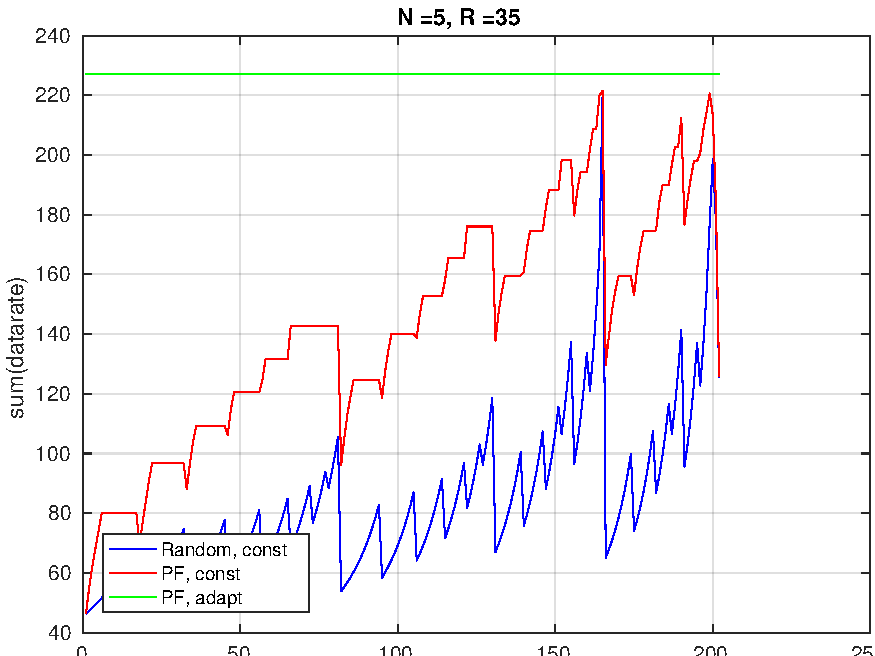
\includegraphics[width=0.6\linewidth]{./pic/circle2_n_5_r_35_sumthr.pdf}
%	\caption{Average OFDMA transmission datarate for $N=5$ and $R=35$}
%	\label{figure:circle_n_5_r_37}
%\end{figure}
%
%\begin{figure}[!htbp]
%	\centering
%	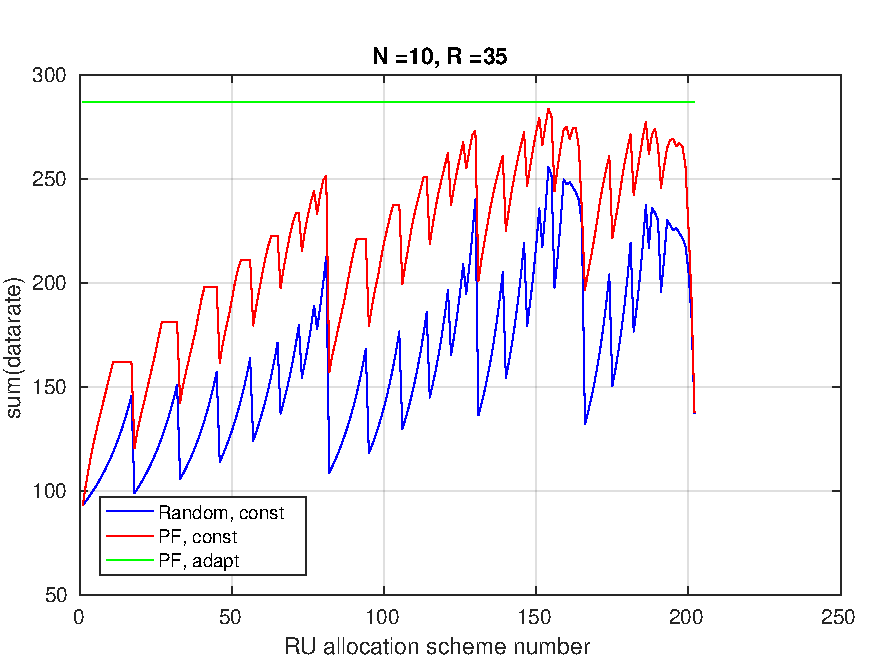
\includegraphics[width=0.6\linewidth]{./pic/circle2_n_10_r_35_sumthr.pdf}
%	\caption{Average OFDMA transmission datarate for $N=10$ and $R=35$}
%	\label{figure:circle_n_10_r_37}
%\end{figure}
%
%\begin{figure}[!htbp]
%	\centering
%	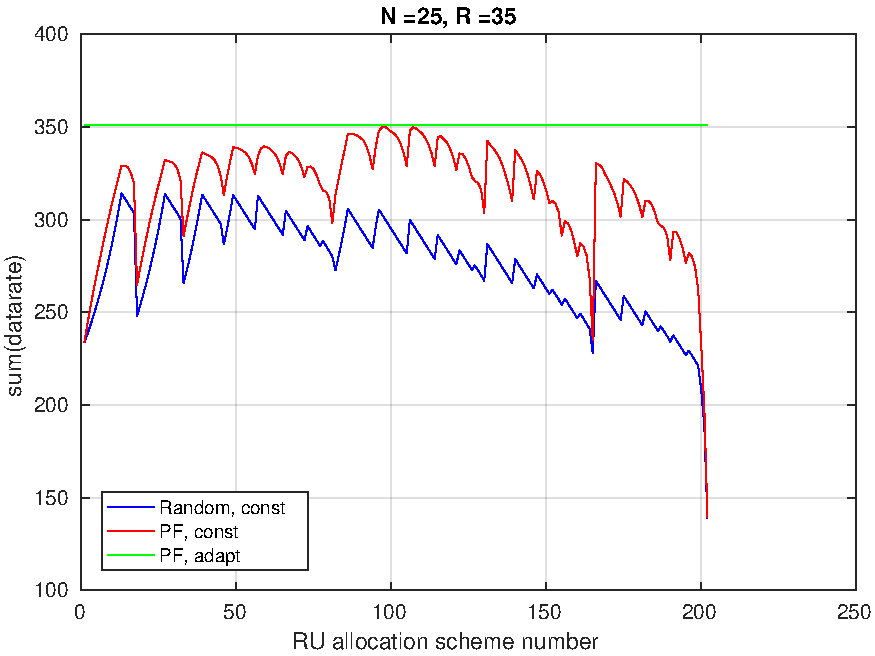
\includegraphics[width=0.6\linewidth]{./pic/circle2_n_25_r_35_sumthr.pdf}
%	\caption{Average OFDMA transmission datarate for $N=25$ and $R=35$}
%	\label{figure:circle_n_25_r_37}
%\end{figure}
%
%\begin{figure}[!htbp]
%	\centering
%	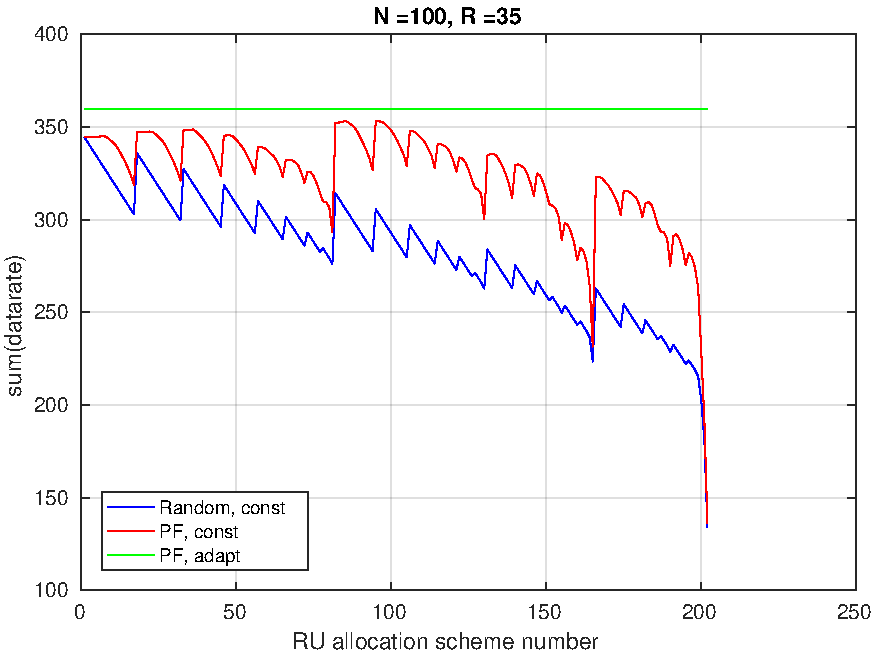
\includegraphics[width=0.6\linewidth]{./pic/circle2_n_100_r_35_sumthr.pdf}
%	\caption{Average OFDMA transmission datarate for $N=100$ and $R=35$}
%	\label{figure:circle_n_100_r_37}
%\end{figure}


%\begin{figure}[!htbp]
%	\centering
%	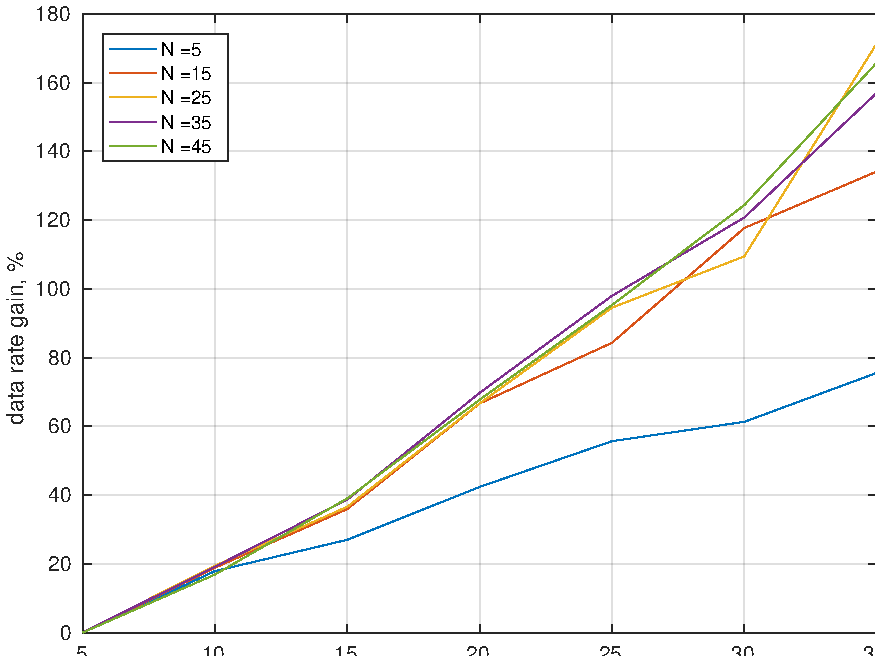
\includegraphics[width=0.6\linewidth]{./pic/thr_gain.pdf}
%	\caption{Data rate gain between PF with dynamic selection of RU configuration and OFDM with random scheduler in Circle scenario}
%	\label{figure:gain}
%\end{figure}
\begin{figure}[!tbp]
	\centering
	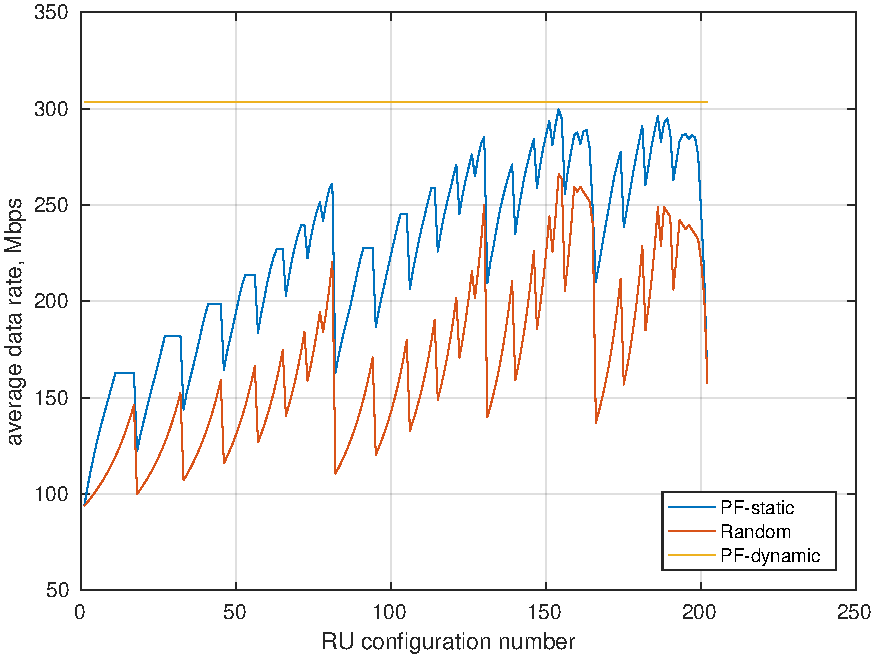
\includegraphics[width=0.6\linewidth]{./pic/n_10.pdf}
	\caption{Average OFDMA transmission data rate achieved with different schedulers for $R=35$ and $N=10$ }
	\label{figure:n_10}
\end{figure}
%\begin{figure}[!htbp]
%	\centering
%	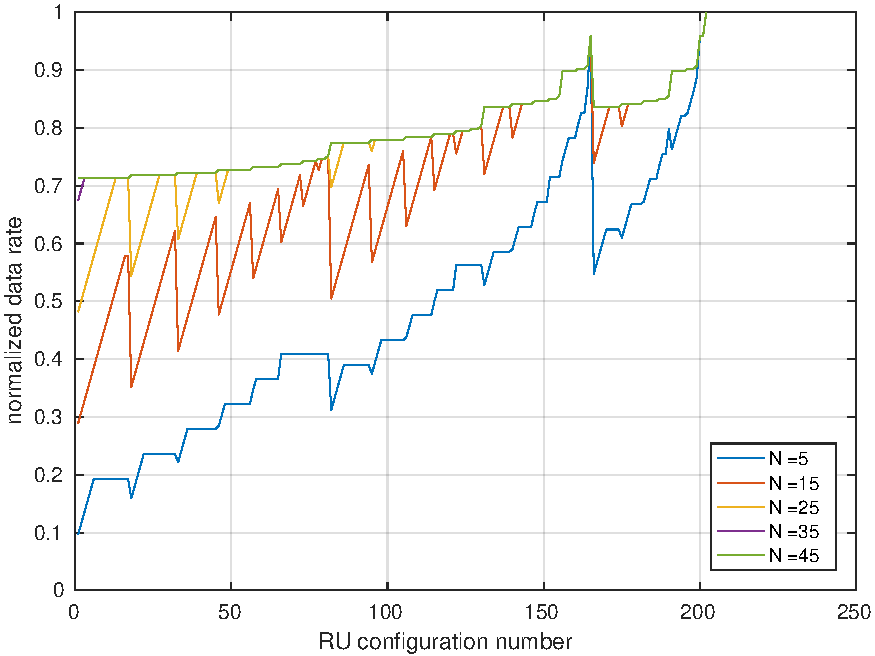
\includegraphics[width=0.6\linewidth]{./pic/r_5.pdf}
%	\caption{Normalized throughput of PF with constant RU configuration for $R=5$ in Circle scenario}
%	\label{figure:r_5}
%\end{figure}
%
%\begin{figure}[!htbp]
%	\centering
%	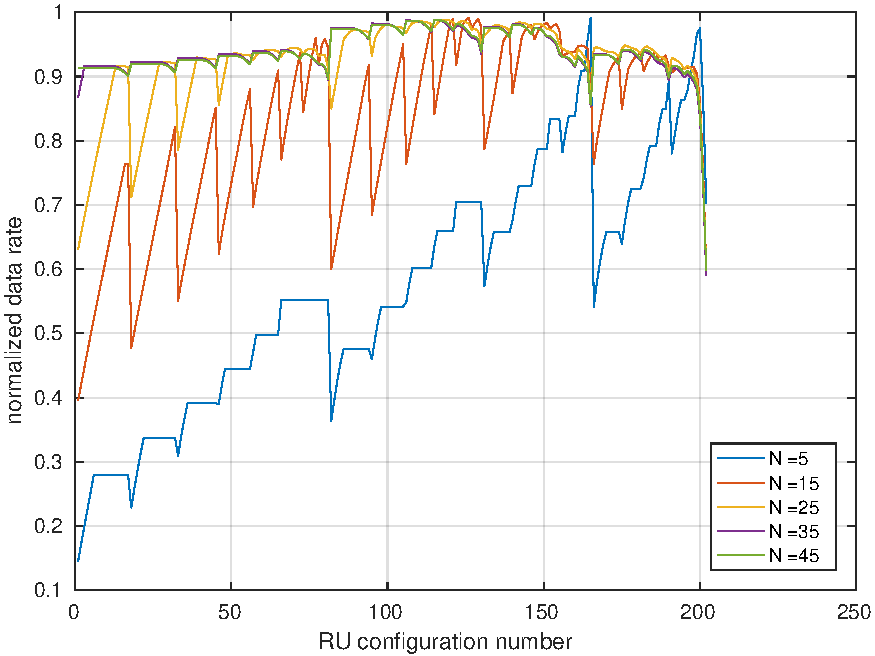
\includegraphics[width=0.6\linewidth]{./pic/r_20.pdf}
%	\caption{Normalized throughput of PF with constant RU configuration for $R=20$ in Circle scenario}
%	\label{figure:r_20}
%\end{figure}

\begin{figure}[!tbp]
	\centering
	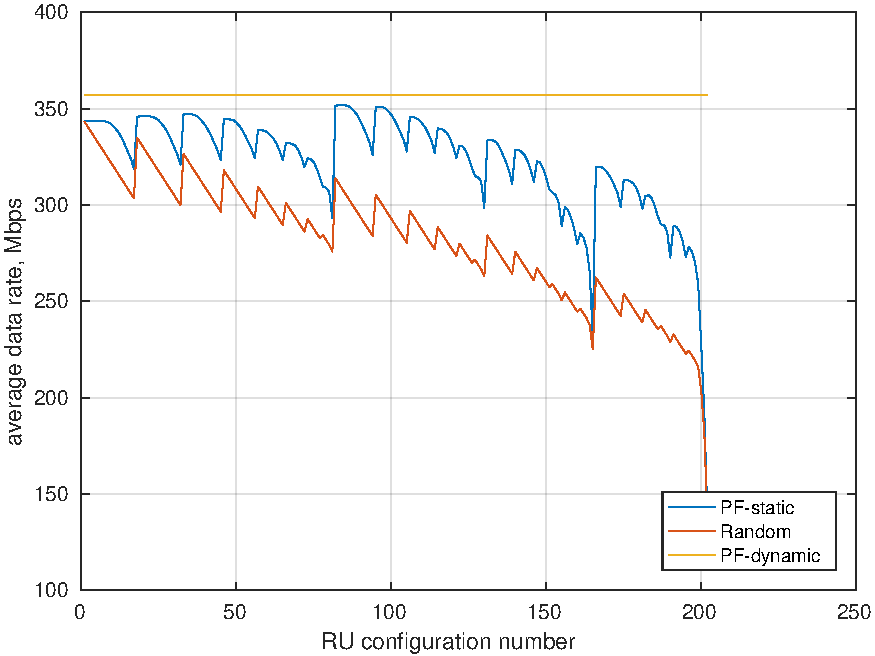
\includegraphics[width=0.6\linewidth]{./pic/n_50.pdf}
	\caption{Average OFDMA transmission data rate achieved with different schedulers for $R=35$ and $N=50$ }
	\label{figure:n_50}
\end{figure}

\section{Conclusion}
\label{sec:conclusion}

In this paper, we study performance of uplink OFDMA in 802.11ax networks with different scheduling algorithms. In future work, we are going to develop a method for dynamic selection of the optimal RU configuration. 

%\section*{Acknowledgment}
%
%The research was supported by the Russian Science Foundation (agreement No 16-19-10687).

\bibliographystyle{IEEEtran}
\bibliography{biblio}


\end{document}             % End of document.